\documentclass{beamer}

\newcommand{\hide}{\onslide+<+(1)->}

\usepackage[utf8]{inputenc}
\usepackage[TS1,T1]{fontenc}
\usepackage[english]{babel}
\usepackage{listings}
\usepackage{xcolor}
\usepackage{tikz}
\usetikzlibrary{backgrounds,decorations.pathreplacing}
\usepackage{mathpartir}
\usepackage{adjustbox}
\usepackage{amsmath}
\usepackage{mathtools}
\usepackage[safe]{tipa} % for \textlambda
\usepackage{wasysym}
\usepackage{stmaryrd}

\usepackage{isabelle}
\usepackage{isabellesym}

\setbeamertemplate{theorems}[normal font]

%\newcommand\pfun{\mathrel{\ooalign{\hfil$\mapstochar\mkern5mu$\hfil\cr$\to$\cr}}}
\newcommand\pfun{\rightharpoonup}

\urlstyle{sf}
\makeatletter
% Inspired by http://anti.teamidiot.de/nei/2009/09/latex_url_slash_spacingkerning/
% but slightly less kern and shorter underscore
% 2013-06-20: Reduced kern for beamer font
\let\UrlSpecialsOld\UrlSpecials
\def\UrlSpecials{\UrlSpecialsOld\do\/{\Url@slash}\do\_{\Url@underscore}}%
\def\Url@slash{\@ifnextchar/{\kern-.01em\mathchar47\kern-.1em}%
   {\kern-.0em\mathchar47\kern-.08em\penalty\UrlBigBreakPenalty}}
\def\Url@underscore{\nfss@text{\leavevmode \kern.06em\vbox{\hrule\@width.3em}}}
\makeatother

\usetheme[titlepage0]{KIT}


\definecolor{light-gray}{gray}{0.95}
\lstdefinestyle{haskell}{
        ,columns=flexible
        ,basewidth={.365em}
        ,keepspaces=True
	,belowskip=0pt
	,backgroundcolor=\color{light-gray}
	,frame=single
	,xleftmargin=2em
	,xrightmargin=2em
        ,basicstyle=\small\sffamily
        ,stringstyle=\itshape
	,language=Haskell
        ,texcl=true
        ,showstringspaces=false
        ,keywords={module,where,import,data,let,in,case,of}
}
\lstnewenvironment{haskell}{\lstset{style=haskell}}{}


\title{Launchbury's Semantik for Lazy Evaluation}
\KITtitleimage[viewport=70 70 300 350]{img}
\subtitle{Research visit at UCM Madrid\\
Joachim Breitner}
\author{Joachim Breitner}
\date{10. \& 11.9.2013}
\iflanguage{ngerman}{%
  \institute{LEHRSTUHL PROGRAMMIERPARADIGMEN}%
}{%
  \institute{PROGRAMMING PARADIGMS GROUP}%
}
\logo{
\includegraphics{Telekom}}


\begin{document}

\maketitle

\begin{frame}
\frametitle{Overview}

\begin{itemize}
\item Who am I?
\item Why am I doing this?
\item What is wrong with correctness, and how to fix it?
\item Launchbury in Isabelle: HOLCF and Nominal
\item What else have I done so far?
\end{itemize}

\end{frame}


\begin{frame}
\frametitle{Who am I?}

\begin{itemize}
\item Studied mathematics and computer science at the University of Karlsruhe.
\item One semester abroad at IIT Bombay.
\item PhD student at the Programming Paradigms Group in Karlsruhe since March 2012.
\item Full scholarship from the Deutsche Telekom Stiftung
\end{itemize}

\end{frame}

\newcommand{\sVar}{\text{Var}}
\newcommand{\sExp}{\text{Exp}}
\newcommand{\sHeap}{\text{Heap}}
\newcommand{\sVal}{\text{Val}}
\newcommand{\sValue}{\text{Value}}
\newcommand{\sEnv}{\text{Env}}
\newcommand{\sApp}[2]{\operatorname{#1}#2}
\newcommand{\sLam}[2]{\text{\textlambda} #1.\, #2}
\newcommand{\sLet}[2]{\text{\textsf{let}}\ #1\ \text{\textsf{in}}\ #2}
\newcommand{\sred}[4]{#1 : #2 \Downarrow #3 : #4}
\newcommand{\sRule}[1]{\text{{\textsc{#1}}}}
\newcommand{\sDeepDup}[1]{\sApp \mdeepDup #1}
\newcommand{\mdeepDup}{\text{\textsf{deepDup}}}
\newcommand{\fv}[1]{\text{fv}(#1)}
\newcommand{\dom}[1]{\text{dom}\,#1}
\newcommand{\fresh}[1]{#1'}

\begin{frame}{Why am I doing this?}%
July 2006: Written an paper on \textit{dup}, a new primitive to duplicate thunks in Haskell; includes a proof with regard to Launchbury's semantics:

\begin{theorem}
Consider the expression
\[
e=\sLet{x_1' = \sDeepDup x_1,\ldots,x_n'= \sDeepDup x_n} e'
\]
with $\fv{e'} \subseteq \{x_1',\ldots,x_n'\}$. If $\sred \Gamma e \Delta z$ and $z$ is a closed value (i.e.\ $\fv{z} = \emptyset$), then $\Gamma \subseteq \Delta$.
\label{thm:deepdup}
\end{theorem}
\pause

After submission of the paper, I thought:
\begin{quote}
“I want to have the proof also in isabelle. Lets quickly formalize Launchbury and prove it.”
\end{quote}
\dots and that is what I’m still doing today.
\end{frame}


\begin{frame}
\frametitle{Terms}

\begin{alignat*}{2}
x,y,u,v,w &\in \sVar
\displaybreak[1]
\\
e &\in
\sExp &&\Coloneqq
\begin{aligned}[t]&
\sLam x e
\mid \sApp e x
\mid x \mid
\\&
\sLet {x_1 = e_1,\ldots,x_n = e_n} e
\end{aligned}
\displaybreak[1]\\
\Gamma, \Delta, \Theta &\in \sHeap &&= \sVar \pfun \sExp
\displaybreak[1]\\
z &\in \sVal &&\Coloneqq \sLam x e
\end{alignat*}
\end{frame}

\begin{frame}
\frametitle{Launchbury’s operational semantics}

\begin{mathpar}
\inferrule
{ }
{\sred{\Gamma}{\sLam xe}{\Gamma}{\sLam xe}}
\sRule{Lam}
\\
\inferrule
{\sred{\Gamma}e{\Delta}{\sLam y e'}\\ \sred{\Delta}{e'[x/y]}{\Theta}{z}}
{\sred\Gamma{\sApp e x}\Theta z}
\sRule{App}
\and
\inferrule
{\sred\Gamma e \Delta z}
{\sred{\Gamma, x\mapsto e} x {\Delta, x\mapsto z}{z}}
\sRule{Var}
\and
\inferrule
{\sred{\Gamma,x_1\mapsto e_1,\ldots,x_n\mapsto e_n} e \Delta z}
{\sred{\Gamma}{\sLet{x_1 = e_1,\ldots, x_n = e_n}e} \Delta z}
\sRule{Let}
\end{mathpar}
\end{frame}


\newcommand{\dsem}[2]{\llbracket #1 \rrbracket_{#2}}
\newcommand{\esem}[1]{\{\!\!\{#1\}\!\!\}}
\newcommand{\rhobot}{\rho\!_\bot}

\begin{frame}
\frametitle{Launchbury’s denotational semantics}

Semantic domain:
\begin{align*}
\sValue &= (\sValue \to \sValue)_\bot &
\sEnv &= \sVar \pfun \sValue
\end{align*}

Meaning of expressions:
\begin{align*}
\dsem{\cdot}{\cdot} &\colon \sExp \to \sEnv \to \sValue \\
\dsem{\sLam xe}{\rho} &=
	%\operatorname{Fn}
	(\lambda v. \dsem{e}{\rho \sqcup \{x \mapsto v\}})\\
\dsem{\sApp e x}\rho &= \dsem e\rho\
	%\downarrow_{\operatorname{Fn}}
	\dsem x \rho \\
\dsem{x}\rho &= \rho (x)\\
\dsem{\sLet{x_1 = e_1,\ldots, x_n = e_n}e}\rho &= \dsem{e}{\esem{ x_1\mapsto e_1,\ldots,x_n\mapsto e_n}\rho}
\end{align*}

Meaning of heaps:
\begin{align*}
\esem{\cdot}\cdot &\colon \sHeap \to \sEnv \to \sEnv \\
\esem{ x_1\mapsto e_1,\ldots,x_n\mapsto e_n}\rho
&= \mu \rho'. \rho \sqcup (x_1 \mapsto \dsem{e_1}{\rho'}) \sqcup \cdots \sqcup (x_n \mapsto \dsem{e_n}{\rho'})\\
\esem{\Gamma} &= \esem{\Gamma}\rhobot
\end{align*}
\end{frame}

\begin{frame}
\frametitle{Launchbury’s ‘Theorem 2’}

Correctness of the operational Semantics:
\[
\sred \Gamma  e \Delta z \implies \dsem{e}{\esem{\Gamma}} = \dsem{z}{\esem{\Delta}}
\]

Generalized to ‘Theorem 2’:
\[
\forall \rho.\ \sred \Gamma  e \Delta z \implies \dsem{e}{\esem{\Gamma}\rho} = \dsem{z}{\esem{\Delta}\rho} \wedge {\esem{\Gamma}\rho} \le \esem{\Delta}\rho
\]

It took me a long time to prove this, \pause and eventually it turned out to be wrong:
\begin{align*}
e &= x & z &= \sLam \_ {\sLet {y = y}y} &  \Gamma = \Delta &= x \mapsto z  & \rho &= x \mapsto \lambda \_.\operatorname{id},
\end{align*}
then
\begin{align*}
\dsem{e}{\esem{\Gamma}\rho} &= \esem{\Gamma}\rho\ (x) = \rho\ (X) \sqcup \dsem{z}{\esem{\Gamma}\rho} = (\lambda \_.\operatorname{id}) \sqcup (\lambda \_.\bot ) =  (\lambda \_.\operatorname{id})\\
\intertext{but}
\dsem{z}{\esem{\Delta}\rho} &= (\lambda \_.\bot ) \ne (\lambda \_.\operatorname{id}).
\end{align*}
\end{frame}

\newcommand{\newstuff}[1]{%
	\onslide<1,3>{{%
	\textcolor<3>{blue}{%
		#1{}%
	}}}%
	}
\begin{frame}
\frametitle{My Semantics}

\begin{mathpar}
\inferrule
{ }
{\sred
{\Gamma}{\newstuff{u \mapsto }\sLam xe \newstuff{, \Gamma'}}
{\Gamma}{\newstuff{u \mapsto {}}\sLam xe \newstuff{, \Gamma'}}
}
\sRule{Lam}
\\
\inferrule
{\sred{\Gamma}{\newstuff{v\mapsto }e\newstuff{,u \mapsto \sApp v x, \Gamma'}}{\Delta}{\newstuff{v \mapsto }\sLam y e'\newstuff{, u \mapsto \sApp v x, \Delta'}}\\
\sred{\Delta}{\newstuff{u \mapsto }e'[x/y]\newstuff{, \Delta'}}{\Theta}{\newstuff{u \mapsto }z\newstuff{, \Theta'}}}
{\sred\Gamma{\newstuff{u \mapsto {}}\sApp e x\newstuff{, \Gamma'}}{\Theta}{\newstuff{u \mapsto }z\newstuff{, \Theta'}}}
\sRule{App}
\and
\inferrule
{\sred\Gamma {\newstuff{x \mapsto }e\newstuff{, u \mapsto x, \Gamma'}}{\Delta}{\newstuff{x \mapsto }z\newstuff{, u \mapsto z, \Delta'}}}
{\sred{\Gamma, x\mapsto e} {\newstuff{u \mapsto }x\newstuff{, \Gamma'}} {\Delta, x\mapsto z}{\newstuff{u \mapsto }z\newstuff{, \Delta'}}}
\sRule{Var}
\and
\inferrule
{\sred{\Gamma,x_1\mapsto e_1,\ldots,x_n\mapsto e_n} {\newstuff{u \mapsto }e\newstuff{, \Gamma'}} \Delta {\newstuff{u \mapsto }z\newstuff{, \Delta'}}}
{\sred{\Gamma}{\newstuff{u \mapsto }\sLet{x_1 = e_1,\ldots, x_n = e_n}e\newstuff{, \Gamma'}} \Delta {\newstuff{u \mapsto }z\newstuff{, \Delta'}}}
\sRule{Let}
\end{mathpar}
\end{frame}

\begin{frame}
\frametitle{My proof of correctness}

As shown in Isabelle, we have:
\[
\sred{\Gamma}{\Gamma'}{\Delta}{\Delta'} \implies \esem{\Gamma, \Gamma'} \le \esem{\Delta, \Delta'}
\]

and hence:

\[
\sred \Gamma  e \Delta z \implies \dsem{e}{\esem{\Gamma}} = \dsem{z}{\esem{\Delta}} \wedge {\esem{\Gamma}} \le \esem{\Delta}.
\]

\pause

\begin{itemize}
\item Isabelle theories published in the Archive of Formal Proofs (\url{http://afp.sf.net/entries/Launchbury.shtml}).
\item Paper write-up submitted to the Journal of Functional Programming (no feedback yet).
\end{itemize}

\end{frame}

\begin{frame}
\frametitle{Formalizing Launchbury: What is Isabelle}

Isabelle/HOL
\begin{itemize}
\item in an interactive theorem prover.
\item builds on Higher Order Logic (simple non-empty types, total functions).
\item is an LCF-style prover.
\item has a large library.
\item Non-trivial definitions (recursive functions, inductive predicates) are not axiomatic, but the objects are constructed explicitly (least fixed points etc) by the corresponding tool.
\end{itemize}

(We will see lots of Isabelle soon.)

\end{frame}

\begin{frame}
\frametitle{Formalizing Launchbury: Ingredience}
We need to
\begin{enumerate}
\item define the terms of the language, and think about name binding.
\item define the operational semantics, which is an inductive predicate.
\item construct the semantic domain for the denotational semantics.
\item define the denotational semantics, by pattern matching on the terms and general recursion.
\item do proofs.
\end{enumerate}

\end{frame}

\begin{frame}
\frametitle{Formalizing Launchbury: Terms}

We could use Launchbury's definition directly and use a plain Isabelle/HOL datatype for terms.\\
But then we’d have to worry a lot about renaming, variable capture etc.

\pause
\bigskip

Better: Use existing tools for that! I use the Nominal package by Christian Urban, based on Nominal Logic by Andrew Pitts. This package provides 

\begin{itemize}
\item data types turned into alpha-equivalence classes.
\item defining functions over these types, by giving equations for a representative element.
\item doing induction over the terms, where the representative elements are chosen by Nominal to avoid certain values.
\end{itemize}

\begin{center}
Demonstration: \texttt{NominalExample.thy}.
\end{center}
\end{frame}



\begin{frame}
\frametitle{Formalizing Launchbury: Heaps}

Options in formalizing heaps

\begin{itemize}
\item Lists of Variable-Term pairs
\begin{itemize}
\item[$\oplus$] Nice syntax
\item[$\oplus$] Good automation
\item[$\ominus$] Need to worry about permutations
\item[$\ominus$] Too much detail, not extensional
\end{itemize}
\item Partial maps 
\begin{itemize}
\item[$\oplus$] Captures meaning precisely
\item[$\ominus$] Not necessarily finite, problems with Nominal.
\end{itemize}
\item Finite partial maps 
\begin{itemize}
\item[$\oplus$] Works
\item[$\ominus$] Need to re-state a number of lemmas 
\item[$\ominus$] Difficult partial order
\end{itemize}
\end{itemize}

(Same issues arise with the denotational semantics of heaps.)
\end{frame}

\begin{frame}
\frametitle{Formalizing Launchbury: Operational Semantics}

\begin{itemize}
\item Straight-forward inductive predicate:

\begin{isabelle}
\isacommand{inductive}\isamarkupfalse%
\isanewline
\ \ reds\ {\isacharcolon}{\isacharcolon}\ {\isachardoublequoteopen}heap\ {\isasymRightarrow}\ exp\ {\isasymRightarrow}\ var\ list\ {\isasymRightarrow}\ heap\ {\isasymRightarrow}\ exp\ {\isasymRightarrow}\ bool{\isachardoublequoteclose}\isanewline
\ \ {\isacharparenleft}{\isachardoublequoteopen}{\isacharunderscore}\ {\isacharcolon}\ {\isacharunderscore}\ {\isasymDown}\isactrlbsub {\isacharunderscore}\isactrlesub \ {\isacharunderscore}\ {\isacharcolon}\ {\isacharunderscore}{\isachardoublequoteclose}\ {\isacharbrackleft}{\isadigit{5}}{\isadigit{0}}{\isacharcomma}{\isadigit{5}}{\isadigit{0}}{\isacharcomma}{\isadigit{5}}{\isadigit{0}}{\isacharcomma}{\isadigit{5}}{\isadigit{0}}{\isacharbrackright}\ {\isadigit{5}}{\isadigit{0}}{\isacharparenright}\isanewline
\isakeyword{where}\isanewline
\ \ Lambda{\isacharcolon}%\isanewline
\ {\isachardoublequoteopen}{\isasymGamma}\ {\isacharcolon}\ {\isacharparenleft}Lam\ {\isacharbrackleft}x{\isacharbrackright}{\isachardot}\ e{\isacharparenright}\ {\isasymDown}\isactrlbsub L\isactrlesub \ {\isasymGamma}\ {\isacharcolon}\ {\isacharparenleft}Lam\ {\isacharbrackleft}x{\isacharbrackright}{\isachardot}\ e{\isacharparenright}{\isachardoublequoteclose}\ \isanewline
%\ {\isacharbar}\ Application{\isacharcolon}\ {\isachardoublequoteopen}{\isasymlbrakk}\isanewline
%\ \ \ \ atom\ y\ {\isasymsharp}\ {\isacharparenleft}{\isasymGamma}{\isacharcomma}e{\isacharcomma}x{\isacharcomma}L{\isacharcomma}{\isasymDelta}{\isacharcomma}{\isasymTheta}{\isacharcomma}z{\isacharparenright}\ {\isacharsemicolon}\isanewline
%\ \ \ \ {\isasymGamma}\ {\isacharcolon}\ e\ {\isasymDown}\isactrlbsub x{\isacharhash}L\isactrlesub \ {\isasymDelta}\ {\isacharcolon}\ {\isacharparenleft}Lam\ {\isacharbrackleft}y{\isacharbrackright}{\isachardot}\ e{\isacharprime}{\isacharparenright}{\isacharsemicolon}\isanewline
%\ \ \ \ {\isasymDelta}\ {\isacharcolon}\ e{\isacharprime}{\isacharbrackleft}y\ {\isacharcolon}{\isacharcolon}{\isacharequal}\ x{\isacharbrackright}\ {\isasymDown}\isactrlbsub L\isactrlesub \ {\isasymTheta}\ {\isacharcolon}\ z\isanewline
%\ \ {\isasymrbrakk}\ \ {\isasymLongrightarrow}\isanewline
%\ \ \ \ {\isasymGamma}\ {\isacharcolon}\ App\ e\ x\ {\isasymDown}\isactrlbsub L\isactrlesub \ {\isasymTheta}\ {\isacharcolon}\ z{\isachardoublequoteclose}\ \isanewline
[..]
%\ {\isacharbar}\ Variable{\isacharcolon}\ {\isachardoublequoteopen}{\isasymlbrakk}\isanewline
%\ \ \ \ {\isacharparenleft}x{\isacharcomma}e{\isacharparenright}\ {\isasymin}\ set\ {\isasymGamma}{\isacharsemicolon}\ delete\ x\ {\isasymGamma}\ {\isacharcolon}\ e\ {\isasymDown}\isactrlbsub x{\isacharhash}L\isactrlesub \ {\isasymDelta}\ {\isacharcolon}\ z\isanewline
%\ \ {\isasymrbrakk}\ {\isasymLongrightarrow}\isanewline
%\ \ \ \ {\isasymGamma}\ {\isacharcolon}\ Var\ x\ {\isasymDown}\isactrlbsub L\isactrlesub \ {\isacharparenleft}x{\isacharcomma}\ z{\isacharparenright}\ {\isacharhash}\ {\isasymDelta}\ {\isacharcolon}\ z{\isachardoublequoteclose}\isanewline
%\ {\isacharbar}\ Let{\isacharcolon}\ {\isachardoublequoteopen}{\isasymlbrakk}\isanewline
%\ \ \ \ set\ {\isacharparenleft}bn\ as{\isacharparenright}\ {\isasymsharp}{\isacharasterisk}\ {\isacharparenleft}{\isasymGamma}{\isacharcomma}\ L{\isacharparenright}{\isacharsemicolon}\isanewline
%\ \ \ \ distinctVars\ {\isacharparenleft}asToHeap\ as{\isacharparenright}{\isacharsemicolon}\isanewline
%\ \ \ \ asToHeap\ as\ {\isacharat}\ {\isasymGamma}\ {\isacharcolon}\ body\ {\isasymDown}\isactrlbsub L\isactrlesub \ {\isasymDelta}\ {\isacharcolon}\ z\isanewline
%\ \ {\isasymrbrakk}\ {\isasymLongrightarrow}\isanewline
%\ \ \ \ {\isasymGamma}\ {\isacharcolon}\ Let\ as\ body\ {\isasymDown}\isactrlbsub L\isactrlesub \ {\isasymDelta}\ {\isacharcolon}\ z{\isachardoublequoteclose}\isanewline
\end{isabelle}

\item Freshness of $y$ in \sRule{Application} and variables in \sRule{Let} demanded.
\item See \texttt{Launchbury.thy} for full definition and basic lemmas.
\item Additional definition with \isa{distinctive} predicates everywere
\end{itemize}

\end{frame}

\begin{frame}
\frametitle{Formalizing Launchbury: Stacked Operational Semantics}

Defined analogously:

\begin{isabelle}
\isacommand{inductive}\isamarkupfalse%
\ reds\ {\isacharcolon}{\isacharcolon}\ {\isachardoublequoteopen}heap\ {\isasymRightarrow}\ heap\ {\isasymRightarrow}\ heap\ {\isasymRightarrow}\ heap\ {\isasymRightarrow}\ bool{\isachardoublequoteclose}\isanewline
\ \ \ {\isacharparenleft}{\isachardoublequoteopen}{\isacharunderscore}\ {\isacharcolon}\ {\isacharunderscore}\ {\isasymDown}\ {\isacharunderscore}\ {\isacharcolon}\ {\isacharunderscore}{\isachardoublequoteclose}\ {\isacharbrackleft}{\isadigit{5}}{\isadigit{0}}{\isacharcomma}{\isadigit{5}}{\isadigit{0}}{\isacharcomma}{\isadigit{5}}{\isadigit{0}}{\isacharcomma}{\isadigit{5}}{\isadigit{0}}{\isacharbrackright}\ {\isadigit{5}}{\isadigit{0}}{\isacharparenright}\isanewline
\isakeyword{where}\isanewline
\ \ Lambda{\isacharcolon}\ {\isachardoublequoteopen}{\isasymGamma}\ {\isacharcolon}\ {\isacharparenleft}x{\isacharcomma}\ {\isacharparenleft}Lam\ {\isacharbrackleft}y{\isacharbrackright}{\isachardot}\ e{\isacharparenright}{\isacharparenright}\ {\isacharhash}\ {\isasymGamma}{\isacharprime}\ {\isasymDown}\ {\isasymGamma}\ {\isacharcolon}\ {\isacharparenleft}x{\isacharcomma}\ {\isacharparenleft}Lam\ {\isacharbrackleft}y{\isacharbrackright}{\isachardot}\ e{\isacharparenright}{\isacharparenright}\ {\isacharhash}\ {\isasymGamma}{\isacharprime}{\isachardoublequoteclose}
\end{isabelle}

(See \texttt{LaunchburyStacked.thy})

\end{frame}



\begin{frame}
\frametitle{Formalizing Launchbury: Denotational Domain}

\begin{itemize}
\item Domain construction using HOLCF:
\begin{isabelle}
\isacommand{domain}\isamarkupfalse%
\ Value\ {\isacharequal}\ Fn\ {\isacharparenleft}\isakeyword{lazy}\ {\isachardoublequoteopen}Value\ {\isasymrightarrow}\ Value{\isachardoublequoteclose}{\isacharparenright}
\end{isabelle}
Defines a new type \isa{Value}, consisting of $\bot$ and $Fn\ f$ where $f$ is of type \isa{Value\ {\isasymrightarrow} Value}, the type of \emph{continuous} functions. Provides \emph{take-induction}.
\item We also define the projection:
\begin{isabelle}
\isacommand{fixrec}\isamarkupfalse%
\ Fn{\isacharunderscore}project\ {\isacharcolon}{\isacharcolon}\ {\isachardoublequoteopen}Value\ {\isasymrightarrow}\ Value\ {\isasymrightarrow}\ Value{\isachardoublequoteclose}\isanewline
\ \isakeyword{where}\ {\isachardoublequoteopen}Fn{\isacharunderscore}project{\isasymcdot}{\isacharparenleft}Fn{\isasymcdot}f{\isacharparenright}{\isasymcdot}v\ {\isacharequal}\ f\ {\isasymcdot}\ v{\isachardoublequoteclose}\isanewline
\isanewline
\isacommand{abbreviation}\isamarkupfalse%
\ Fn{\isacharunderscore}project{\isacharunderscore}abbr\ {\isacharparenleft}\isakeyword{infix}\ {\isachardoublequoteopen}{\isasymdown}Fn{\isachardoublequoteclose}\ {\isadigit{5}}{\isadigit{5}}{\isacharparenright}\isanewline
\ \ \isakeyword{where}\ {\isachardoublequoteopen}f\ {\isasymdown}Fn\ v\ {\isasymequiv}\ Fn{\isacharunderscore}project{\isasymcdot}f{\isasymcdot}v{\isachardoublequoteclose}\isanewline
\end{isabelle}
\end{itemize}
\end{frame}

\begin{frame}
\frametitle{Formalizing Launchbury: Heap denotation}

\begin{itemize}
\item Defined as taking the expression semantics as an parameter, can be used for $\dsem{\_}\_$ and $\mathcal N\dsem{\_}\_$.
\item Hairy issue 1:
\begin{itemize}
\item $\sqcup$ is on \isa{Value} not always defined.
\item Therefore, the heap semantics is a partial function.
\end{itemize}
$\implies$ custom predicate on when all joins in ($\mu \rho'.\,\rho \sqcup f \rho'$ )are defined.
\item Hairy issue 2:
\begin{itemize}
\item Heap semantics are \emph{finite} maps, for Nominal's needs.
\item \emph{Finite} maps are not chain-complete, so cannot use HOLCF's $\mu$-operator.
\item Cannot put the domain in the type, as HOL is not depdently types.
\end{itemize}
$\implies$ custom theory of pcpo on explicit carrier sets.
\item All in all lots of technical problems, and hardly needed, as usually the domains are disjoint.
\end{itemize}
\end{frame}

\begin{frame}
\frametitle{Formalizing Launchbury: Heap denotation}

\begin{itemize}
\item Defines using \isa{\isacommand{nominal{\isacharunderscore}primrec}}:
\begin{isabelle}
\isacommand{nominal{\isacharunderscore}primrec}\isamarkupfalse%
\isanewline
\ \ ESem\ {\isacharcolon}{\isacharcolon}\ {\isachardoublequoteopen}exp\ {\isasymRightarrow}\ Env\ {\isasymRightarrow}\ Value{\isachardoublequoteclose}\ {\isacharparenleft}{\isachardoublequoteopen}{\isasymlbrakk}{\isacharunderscore}{\isasymrbrakk}\isactrlbsub {\isacharunderscore}\isactrlesub {\isachardoublequoteclose}\ \ {\isacharbrackleft}{\isadigit{6}}{\isadigit{0}}{\isacharcomma}{\isadigit{6}}{\isadigit{0}}{\isacharbrackright}\ {\isadigit{6}}{\isadigit{0}}{\isacharparenright}\isanewline
\isakeyword{where}\isanewline
\ \ {\isachardoublequoteopen}atom\ x\ {\isasymsharp}\ {\isasymrho}\ {\isasymLongrightarrow}\isanewline
\ \ {\isasymlbrakk}\ Lam\ {\isacharbrackleft}x{\isacharbrackright}{\isachardot}\ e\ {\isasymrbrakk}\isactrlbsub {\isasymrho}\isactrlesub \ {\isacharequal}\ Fn\ {\isasymcdot}\ {\isacharparenleft}{\isasymLambda}\ v{\isachardot}\ {\isacharparenleft}{\isasymlbrakk}\ e\ {\isasymrbrakk}\isactrlbsub {\isasymrho}{\isacharparenleft}x\ f{\isasymmapsto}\ v{\isacharparenright}\isactrlesub {\isacharparenright}{\isacharparenright}{\isachardoublequoteclose}\isanewline
{\isacharbar}\ {\isachardoublequoteopen}{\isasymlbrakk}\ App\ e\ x\ {\isasymrbrakk}\isactrlbsub {\isasymrho}\isactrlesub \ {\isacharequal}\ {\isasymlbrakk}\ e\ {\isasymrbrakk}\isactrlbsub {\isasymrho}\isactrlesub \ {\isasymdown}Fn\ {\isasymlbrakk}\ Var\ x\ {\isasymrbrakk}\isactrlbsub {\isasymrho}\isactrlesub{\isachardoublequoteclose}\isanewline
{\isacharbar}\ {\isachardoublequoteopen}{\isasymlbrakk}\ Var\ x\ {\isasymrbrakk}\isactrlbsub {\isasymrho}\isactrlesub \ {\isacharequal}\ {\isasymrho}\ f{\isacharbang}\ x{\isachardoublequoteclose}\isanewline
{\isacharbar}\ {\isachardoublequoteopen}set\ {\isacharparenleft}bn\ as{\isacharparenright}\ {\isasymsharp}{\isacharasterisk}\ {\isasymrho}\ {\isasymLongrightarrow}\isanewline
\ \ {\isasymlbrakk}\ Let\ as\ body\ {\isasymrbrakk}\isactrlbsub {\isasymrho}\isactrlesub \ {\isacharequal}\ {\isasymlbrakk}body{\isasymrbrakk}\isactrlbsub has{\isacharunderscore}ESem{\isachardot}HSem\ ESem\ {\isacharparenleft}asToHeap\ as{\isacharparenright}\ {\isasymrho}\isactrlesub {\isachardoublequoteclose}
\end{isabelle}
\item Shown to be continuous
\item \isa{{\isachardoublequoteopen}x\ {\isasymnoteq}\ y\ {\isasymLongrightarrow}\ atom\ x\ {\isasymsharp}\ {\isasymrho}\ {\isasymLongrightarrow}\ \ {\isasymlbrakk}\ e\ {\isasymrbrakk}\isactrlbsub {\isasymrho}{\isacharparenleft}x\ f{\isasymmapsto}\ {\isasymlbrakk}Var\ y{\isasymrbrakk}\isactrlbsub {\isasymrho}\isactrlesub {\isacharparenright}\isactrlesub \ {\isacharequal}\ {\isasymlbrakk}\ e{\isacharbrackleft}x{\isacharcolon}{\isacharcolon}{\isacharequal}\ y{\isacharbrackright}\ {\isasymrbrakk}\isactrlbsub {\isasymrho}\isactrlesub {\isachardoublequoteclose}}
\item Fresh variables in \isa{\isasymrho} do not affect \isa{{\isasymlbrakk}e{\isasymrbrakk}\isactrlbsub {\isasymrho}\isactrlesub }
\item {\ldots} and a few lemmas more.
\end{itemize}
\end{frame}

\begin{frame}
\frametitle{Correctness Proof}

\begin{itemize}
\item Main proof towards correctness (no generalization needed!):
\begin{isabelle}
\isacommand{theorem}\isamarkupfalse%
\ correctness{\isacharcolon}\isanewline
\ \ \isakeyword{assumes}\ {\isachardoublequoteopen}{\isasymGamma}\ {\isacharcolon}\ {\isasymGamma}{\isacharprime}\ {\isasymDown}\ {\isasymDelta}\ {\isacharcolon}\ {\isasymDelta}{\isacharprime}{\isachardoublequoteclose}\isanewline
\ \ \isakeyword{and}\ {\isachardoublequoteopen}distinctVars\ {\isacharparenleft}{\isasymGamma}{\isacharprime}\ {\isacharat}\ {\isasymGamma}{\isacharparenright}{\isachardoublequoteclose}\isanewline
\ \ \isakeyword{shows}\ {\isachardoublequoteopen}{\isasymlbrace}{\isasymGamma}{\isacharprime}{\isacharat}{\isasymGamma}{\isasymrbrace}\ {\isasymle}\ {\isasymlbrace}{\isasymDelta}{\isacharprime}{\isacharat}{\isasymDelta}{\isasymrbrace}{\isachardoublequoteclose}
\end{isabelle}
\item Equivalency of the operational semantics
\begin{isabelle}
\isacommand{lemma}\isamarkupfalse%
\ add{\isacharunderscore}stack{\isacharcolon}\isanewline
\ \ \isakeyword{assumes}\ {\isachardoublequoteopen}{\isasymGamma}\ {\isacharcolon}\ e\ {\isasymDown}\isactrlbsub L\isactrlesub \ {\isasymDelta}\ {\isacharcolon}\ z{\isachardoublequoteclose}\isanewline
\ \ \isakeyword{assumes}\ {\isachardoublequoteopen}x\ {\isasymin}\ set\ L{\isachardoublequoteclose}\isanewline
\ \ \isakeyword{assumes}\ {\isachardoublequoteopen}supp\ {\isasymGamma}{\isacharprime}\ {\isasymsubseteq}\ supp\ L{\isachardoublequoteclose}\isanewline
\ \ \isakeyword{shows}\ {\isachardoublequoteopen}{\isasymGamma}\ {\isacharcolon}\ {\isacharparenleft}x{\isacharcomma}e{\isacharparenright}\ {\isacharhash}\ {\isasymGamma}{\isacharprime}\ {\isasymDown}\ {\isasymDelta}\ {\isacharcolon}\ {\isacharparenleft}x{\isacharcomma}z{\isacharparenright}\ {\isacharhash}\ {\isasymGamma}{\isacharprime}{\isachardoublequoteclose}
\end{isabelle}
\item Finally\dots
\begin{isabelle}
\isacommand{theorem}\isamarkupfalse%
\ correctness{\isacharcolon}\isanewline
\ \ \isakeyword{assumes}\ {\isachardoublequoteopen}{\isasymGamma}\ {\isacharcolon}\ e\ {\isasymDown}\isactrlbsub L\isactrlesub \ {\isasymDelta}\ {\isacharcolon}\ z{\isachardoublequoteclose} \isakeyword{and} {\isachardoublequoteopen}distinctVars\ {\isasymGamma}{\isachardoublequoteclose}\isanewline
\ \ \isakeyword{shows}\ {\isachardoublequoteopen}{\isasymlbrakk}e{\isasymrbrakk}\isactrlbsub {\isasymlbrace}{\isasymGamma}{\isasymrbrace}\isactrlesub \ {\isacharequal}\ {\isasymlbrakk}z{\isasymrbrakk}\isactrlbsub {\isasymlbrace}{\isasymDelta}{\isasymrbrace}\isactrlesub {\isachardoublequoteclose}\ \isakeyword{and}\ {\isachardoublequoteopen}{\isasymlbrace}{\isasymGamma}{\isasymrbrace}\ {\isasymle}\ {\isasymlbrace}{\isasymDelta}{\isasymrbrace}{\isachardoublequoteclose}
\end{isabelle}
\end{itemize}
\end{frame}

\begin{frame}
\frametitle{Sidetrack:\\ Update-based denotational semantics}

\begin{itemize}
\item One can take $\sqcup$ in the denotational demantics to mean right-sided update
\item Then things become easy:
\begin{itemize}
\item the operation is always defined
\item the original proof goes through
\item the semantics agree on terms, and on heaps that are disjoint with the environment.
\end{itemize}
(see \texttt{DenotationalEquivalences})
\item \dots but for us, the denotational semantics is the specification, so we do not want to change it nilly-willy.
\end{itemize}
\end{frame}

\begin{frame}
\frametitle{Since then: Resourced semantics}

\begin{itemize}
\item Definition of the resourced semantics domain (\texttt{CValue.thy})
\item Definition of the similarity relation (\texttt{ValueSimilarity})
\item Definition the resourced semantics (\texttt{ResourcedDenotational})
\item Equivalency of the two semantics:
\begin{isabelle}
\ \ \isakeyword{assumes}\ {\isachardoublequoteopen}{\isasymrho}\ f{\isasymtriangleleft}{\isasymtriangleright}\ {\isasymsigma}{\isachardoublequoteclose}\isanewline
\ \ \isakeyword{shows}\ {\isachardoublequoteopen}{\isasymlbrakk}e{\isasymrbrakk}\isactrlbsub {\isasymrho}\isactrlesub \ {\isasymtriangleleft}{\isasymtriangleright}\ {\isacharparenleft}{\isasymN}{\isasymlbrakk}e{\isasymrbrakk}\isactrlbsub {\isasymsigma}\isactrlesub {\isacharparenright}{\isasymcdot}{\isacharparenleft}C\isactrlsup {\isasyminfinity}{\isacharparenright}{\isachardoublequoteclose}
\end{isabelle}
(two \isa{\isacommand{sorry}}s left: Semantics of undefined variables, and Nominal's proof obligations for the resourced semantics.)
\end{itemize}
\end{frame}

\begin{frame}
\frametitle{Since then: Towards removing indirections}

Modified the operational semantics again:

\begin{isabelle}
\isacommand{inductive}\isamarkupfalse\ reds\isanewline
\ \ {\isacharcolon}{\isacharcolon}\ {\isachardoublequoteopen}Heap\ {\isasymRightarrow}\ Flag\ {\isasymRightarrow}\ Flag\ {\isasymRightarrow}\ Flag\ {\isasymRightarrow}\ var\ list\ {\isasymRightarrow}\ Heap\ {\isasymRightarrow}\ bool{\isachardoublequoteclose}\isanewline
\ \ \ \ {\isacharparenleft}{\isachardoublequoteopen}{\isacharunderscore}{\isacharslash}\ {\isasymDown}\isactrlsup {\isacharunderscore}\isactrlsup {\isacharunderscore}\isactrlsup {\isacharunderscore}\isactrlbsub {\isacharunderscore}\isactrlesub {\isacharslash}\ {\isacharunderscore}{\isachardoublequoteclose}\ {\isacharbrackleft}{\isadigit{5}}{\isadigit{0}}{\isacharcomma}{\isadigit{5}}{\isadigit{0}}{\isacharcomma}{\isadigit{5}}{\isadigit{0}}{\isacharcomma}{\isadigit{5}}{\isadigit{0}}{\isacharcomma}{\isadigit{5}}{\isadigit{0}}{\isacharbrackright}\ {\isadigit{5}}{\isadigit{0}}{\isacharparenright}
\end{isabelle}
\begin{itemize}
\item Flags to disable/enable specific rules: Indirections on/off, updates on/off (not yet in final form), blackholing on/off.
\item Heaps as finite maps instead of lists.
\item Stack as a list of variables, with expressions still on the heap.
\item Minor cheating in \sRule{Application}: Leaves a useless binding on the heap
\item TODO: Equivalency to the original semantics.
\item Possibly not the best form for adequacy, as the heap keeps changing.
\end{itemize}
\end{frame}

\begin{frame}
\frametitle{Indirections}
\begin{itemize}
\item Defined Indirections:
\begin{isabelle}
\isacommand{type{\isacharunderscore}synonym}\isamarkupfalse%
\ indirections\ {\isacharequal}\ {\isachardoublequoteopen}{\isacharparenleft}var\ {\isasymtimes}\ var{\isacharparenright}\ list{\isachardoublequoteclose}
\end{isabelle}
\item Notion of valid indirections (acyclic)
\item Notion of compatible indirections:
\begin{isabelle}
\isacommand{definition}\isamarkupfalse%
\ ind{\isacharunderscore}for\ {\isacharcolon}{\isacharcolon}\ {\isachardoublequoteopen}indirections\ {\isasymRightarrow}\ Heap\ {\isasymRightarrow}\ bool{\isachardoublequoteclose}\ \isakeyword{where}\isanewline
\ \ {\isachardoublequoteopen}ind{\isacharunderscore}for\ is\ {\isasymGamma}\ {\isacharequal}\ {\isacharparenleft}{\isasymforall}\ {\isacharparenleft}x{\isacharcomma}y{\isacharparenright}\ {\isasymin}\ set\ is{\isachardot}\ {\isacharparenleft}x\ {\isasymin}\ fdom\ {\isasymGamma}\ {\isasymand}\ {\isacharparenleft}{\isacharparenleft}{\isacharparenleft}lookup\ {\isasymGamma}\ x{\isacharparenright}\ {\isacharequal}\ Some\ {\isacharparenleft}Var\ y{\isacharparenright}\ {\isasymor}\ {\isacharparenleft}isLam\ {\isacharparenleft}{\isasymGamma}\ f{\isacharbang}\ x{\isacharparenright}{\isacharparenright}\ {\isasymand}\ lookup\ {\isasymGamma}\ x\ {\isacharequal}\ lookup\ {\isasymGamma}\ y{\isacharparenright}{\isacharparenright}{\isacharparenright}{\isacharparenright}{\isachardoublequoteclose}
\end{isabelle}
Would be easier without updates!
\item Indirection-removing operation ($\ominus$) on
\begin{itemize}
\item variables,
\item expressions,
\item heaps and
\item stacks (which is tricky and made me change how stacks look).
\end{itemize}
\end{itemize}
\end{frame}

\begin{frame}
\frametitle{Since then: Adding blackholing}
\begin{itemize}
\item Made indirection removing easier, and was relatively easy by itself
\item Adding blackholing:
\begin{isabelle}
\isacommand{theorem}\isamarkupfalse%
\isanewline
\ \ \isakeyword{assumes}\ {\isachardoublequoteopen}{\isasymGamma}\ {\isasymDown}\isactrlsup i\isactrlsup u\isactrlsup b\isactrlbsub x{\isacharhash}S\isactrlesub \ {\isasymDelta}{\isachardoublequoteclose}\isanewline
\ \ \isakeyword{assumes}\ {\isachardoublequoteopen}validStack\ {\isasymGamma}\ x\ S{\isachardoublequoteclose}\isanewline
\ \ \isakeyword{shows}\ {\isachardoublequoteopen}{\isasymnot}\ cycle\ {\isasymGamma}\ x{\isachardoublequoteclose}\ \isakeyword{and}\ {\isachardoublequoteopen}validStack\ {\isasymDelta}\ x\ S{\isachardoublequoteclose}\ \isakeyword{and}\ {\isachardoublequoteopen}{\isasymGamma}\ {\isasymDown}\isactrlsup i\isactrlsup u\isactrlsup {\isasymsurd}\isactrlbsub x{\isacharhash}S\isactrlesub \ {\isasymDelta}{\isachardoublequoteclose}
\end{isabelle}
\item And removing them (trivial):
\begin{isabelle}
\isacommand{lemma}\isamarkupfalse%
\ remove{\isacharunderscore}blackholing{\isacharcolon}\isanewline
\ \ \isakeyword{assumes}\ {\isachardoublequoteopen}{\isasymGamma}\ {\isasymDown}\isactrlsup i\isactrlsup u\isactrlsup {\isasymsurd}\isactrlbsub S\isactrlesub \ {\isasymDelta}{\isachardoublequoteclose}\isanewline
\ \ \isakeyword{shows}\ {\isachardoublequoteopen}{\isasymGamma}\ {\isasymDown}\isactrlsup i\isactrlsup u\isactrlsup b\isactrlbsub S\isactrlesub \ {\isasymDelta}{\isachardoublequoteclose}\isanewline
\end{isabelle}
\end{itemize}
\end{frame}

\begin{frame}
\frametitle{Since then: Finally removing indirections}
\begin{itemize}
\item The complete theorem (ugly, and took me too long):
\begin{isabelle}
\isacommand{theorem}\isamarkupfalse%
\ remove{\isacharunderscore}indirection{\isacharprime}{\isacharcolon}\isanewline
\ \ {\isachardoublequoteopen}{\isasymGamma}\ {\isasymDown}\isactrlsup {\isasymsurd}\isactrlsup u\isactrlsup {\isasymtimes}\isactrlbsub S\isactrlesub \ {\isasymDelta}\ {\isasymLongrightarrow}\isanewline
\ \ \ \ ind{\isacharunderscore}for\ is\ {\isasymGamma}\ {\isasymLongrightarrow}\isanewline
\ \ \ \ valid{\isacharunderscore}ind\ is\ {\isasymLongrightarrow}\isanewline
\ \ {\isasymexists}\ is{\isacharprime}{\isachardot}\ {\isacharparenleft}{\isasymGamma}\ {\isasymominus}\isactrlsub H\ is\ {\isasymDown}\isactrlsup {\isasymtimes}\isactrlsup u\isactrlsup {\isasymtimes}\isactrlbsub S\ {\isasymominus}\isactrlsub S\ is\isactrlesub \ {\isasymDelta}\ {\isasymominus}\isactrlsub H\ is{\isacharprime}{\isacharparenright}\isanewline
\ \ \ \ \ \ \ {\isasymand}\ ind{\isacharunderscore}for\ is{\isacharprime}\ {\isasymDelta}\isanewline
\ \ \ \ \ \ \ {\isasymand}\ set\ is\ {\isasymsubseteq}\ set\ is{\isacharprime}\isanewline
\ \ \ \ \ \ \ {\isasymand}\ {\isacharparenleft}heapVars\ is{\isacharprime}\ {\isasyminter}\ fdom\ {\isasymGamma}{\isacharparenright}\ {\isasymsubseteq}\ heapVars\ is\isanewline
\ \ \ \ \ \ \ {\isasymand}\ valid{\isacharunderscore}ind\ is{\isacharprime}\isanewline
\ \ \ \ \ \ \ {\isasymand}\ S\ {\isasymominus}\isactrlsub S\ is{\isacharprime}\ {\isacharequal}\ S\ {\isasymominus}\isactrlsub S\ is{\isachardoublequoteclose}\isanewline
\end{isabelle}

\item The interesting case:
\begin{isabelle}
\isacommand{corollary}\isamarkupfalse%
\ remove{\isacharunderscore}indirection{\isacharcolon}\isanewline
\ \ \isakeyword{assumes}\ {\isachardoublequoteopen}{\isasymGamma}\ {\isasymDown}\isactrlsup {\isasymsurd}\isactrlsup u\isactrlsup {\isasymtimes}\isactrlbsub S\isactrlesub \ {\isasymDelta}{\isachardoublequoteclose}\isanewline
\ \ \isakeyword{shows}\ {\isachardoublequoteopen}{\isasymexists}\ {\isasymDelta}{\isacharprime}{\isachardot}\ {\isasymGamma}\ {\isasymDown}\isactrlsup {\isasymtimes}\isactrlsup u\isactrlsup {\isasymtimes}\isactrlbsub S\isactrlesub \ {\isasymDelta}{\isacharprime}{\isachardoublequoteclose}
\end{isabelle}
\end{itemize}
\end{frame}


\begin{frame}[fragile]
\frametitle{The big picture}

\begin{center}
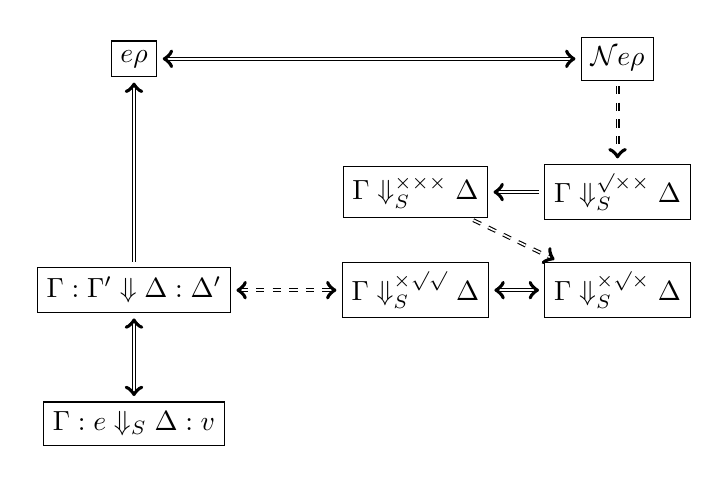
\begin{tikzpicture}[every node/.style={align=center}]
\matrix (m) [row sep=1.5em, column sep=2em] 
{
\node[draw] (ds) {$\dsem{e}\rho$}; && & \node[draw] (rds) {$\mathcal{N}\dsem{e}\rho$}; \\\\
&&
\node[draw] (nnn) {$\Gamma \Downarrow^{\times\times\times}_S \Delta$}; &
\node[draw] (ynn) {$\Gamma \Downarrow^{\surd\times\times}_S \Delta$}; \\

\node[draw] (ss) {$\Gamma : \Gamma' \Downarrow \Delta : \Delta'$};
&&
\node[draw] (nyy) {$\Gamma \Downarrow^{\times\surd\surd}_S \Delta$}; &
\node[draw] (nyn) {$\Gamma \Downarrow^{\times\surd\times}_S \Delta$}; \\\\
\node[draw] (ns) {$\Gamma : e \Downarrow_S \Delta : v$}; \\
};

\small
\draw[<->,double, shorten <=.5ex, shorten >= .5ex] (ds) -- (rds);
\draw[<->,double, shorten <=.5ex, shorten >= .5ex] (ss) -- (ns);
\draw[->,double, shorten <=.5ex, shorten >= .5ex] (ss) -- (ds);
\draw[<->,double, shorten <=.5ex, shorten >= .5ex] (nyy) -- (nyn);
\draw[->,double, shorten <=.5ex, shorten >= .5ex] (ynn) -- (nnn);
\draw[->,dashed,double, shorten <=.5ex, shorten >= .5ex] (rds) -- (ynn);
\draw[->,dashed,double, shorten <=.5ex, shorten >= .5ex] (nnn) -- (nyn);
\draw[<->,dashed,double, shorten <=.5ex, shorten >= .5ex] (ss) -- (nyy);
%\draw[gray,<->,double, shorten <=.5ex, shorten >= .5ex]  (on) -- (mn) node[midway,below] {stated};
%\draw[gray,->,double, shorten <=.5ex, shorten >= .5ex]  (rd) -- (mn) node[midway,right] {proof outlined};
%\draw[gray,<->,double, shorten <=.5ex, shorten >= .5ex]  (rd) -- (jd) node[midway,above] {stated} 
%                                                            node[midway,below] {later proved in \cite{functionspaces}}; \draw[gray,->,double, shorten <=.5ex, shorten >= .5ex] (on) -- (jd) node[midway,left] {proof failed};
%\draw[<->,double, shorten <=.5ex, shorten >= .5ex]  (on) -- (sn) node[midway,above] {formally proved};
%\draw[->,double, shorten <=.5ex, shorten >= .5ex] (sn) -- (jd.east) node[sloped,midway,above] {formally proved};
%%\draw[->,double, shorten <=.5ex, shorten >= .5ex] (on) -- (ud) node[sloped,midway,above] {Proof};
%%\draw[<->,double, shorten <=.5ex, shorten >= .5ex]  (jd) -- (ud) node[midway,below] {formally proved};
%\node[gray] at (barycentric cs:on=1,mn=1,rd=1,jd=1) {\cite{launchbury}};
\end{tikzpicture}
\end{center}
\end{frame}

\begin{frame}
\frametitle{Open questions (for me)}

\begin{itemize}
\item How to modify the operational semantics such that the variant without updates gets nice and the adequacy proof can succeed?
\item Are indirections really required or is it possibly enough to use a substitution lemma on the denotational side?
\item What to do with the formalization when it is done?
\begin{itemize}
\item Extend with GC, data types, primitive types?
\item Prove compiler transformation correct?
\item Write a compiler and prove it correct?
\end{itemize}
\end{itemize}
\end{frame}

\begin{frame}
\begin{center}
¡Muchas gracias!
\end{center}
\end{frame}


\end{document}
